%\documentclass[xcolor={dvipsnames}, handout]{beamer}
\documentclass[xcolor={dvipsnames}]{beamer}

%\setbeamertemplate{footline}[frame number]
%\setbeamersize{description width=-\labelsep}
\usetheme{SimpleDarkBlue}

%\usepackage{amsmath,amsfonts,amssymb,pxfonts,eulervm,xspace}
\usepackage{amsmath, amsfonts, amssymb, mathtools, eulervm, xspace}
\renewcommand{\restriction}{\mathord{\upharpoonright}} %restriction w/p space
\usepackage{relsize} %mathlarger
\usepackage{bm}
\usepackage{centernot}
\usepackage{mathrsfs} % math script fonts
\usepackage{tikz}
\usetikzlibrary{cd} % commutative diagrams
\newtheorem{prop}{Proposition} %math?

\usepackage{subcaption} % subfigure float captioning

\usepackage{tabulary}
\usepackage{tabularx}
%\usepackage{enumitem} $ won't work with beamer
\usepackage{booktabs}
\usepackage{multirow}
\usepackage{array}

\usepackage{graphicx}
\usepackage{adjustbox}%scale tikz-cd

\usepackage{appendixnumberbeamer}
\usepackage{comment}
\usepackage{minted}
\setminted[python]{fontsize=\scriptsize,
                   linenos,
                   numbersep=8pt,
                   autogobble,
                   frame=lines,
                   bgcolor=bg,
                   framesep=3mm}

\usepackage{notation} % move this later

\graphicspath{.figures/, ../papers/figures/}

\usepackage[backend=bibtex, sorting=none, doi=false,isbn=false,url=false, giveninits=true]{biblatex}

\bibliography{references}


\newenvironment{changemargin}[2]{%
\begin{list}{}{%
\setlength{\topsep}{0pt}%
\setlength{\leftmargin}{#1}%
\setlength{\rightmargin}{#2}%
\setlength{\listparindent}{\parindent}%
\setlength{\itemindent}{\parindent}%
\setleng{}th{\parsep}{\parskip}%
}%
\item[]}{\end{list}}

\title{Topologically Equivariant \\ Artist Model}
\author{Hannah Aizenman\texorpdfstring{\\}{,}  Mikael Vejdemo-Johansson \texorpdfstring{\\}{,} Thomas Caswell \texorpdfstring{\\}{,} Michael Grossberg}
\institute{Department of Computer Science, The Graduate Center}
\date{\today}

\begin{document}

\begin{frame}<presentation:1|handout:1>
	\titlepage
    %Hannah Aizenman, Mikael Vejdemo-Johansson, Thomas Caswell, Michael Grossberg\\
    %Committee: Dr. Robert Haralick, Dr. Lev Manovich, Dr. Huy Vo\\
    %External Member: Dr. Marcus Hanwell
\end{frame}

\begin{frame}{About}
    \begin{block}{Me}
        \begin{itemize}
            \item PhD candidate in Computer Science
            \item Matplotlib Community Manager \& Core Developer
            \item  socials/github: story645
        \end{itemize}
    \end{block}

    \begin{block}{Project}
        \begin{itemize}
            \item Funded by Chan Zuckerberg Initiative EOSS 1 \& 3
        \end{itemize}
    \end{block}
\end{frame}

\section{Introduction}
\begin{frame}{Goals}
    \begin{itemize}
        \item uniform API for arbitrary datasets in arbitrary data containers
        \item generalizable methodology for expressing structure preservation
        \item framework that translates into coding specifications
    \end{itemize}
\end{frame}


%% maybe pull out the middle for now? move the 3 stages down to construction?
\begin{frame}{What do visualization libraries do?}
    \begin{figure}
        \begin{overprint}
            \onslide<1|handout:1>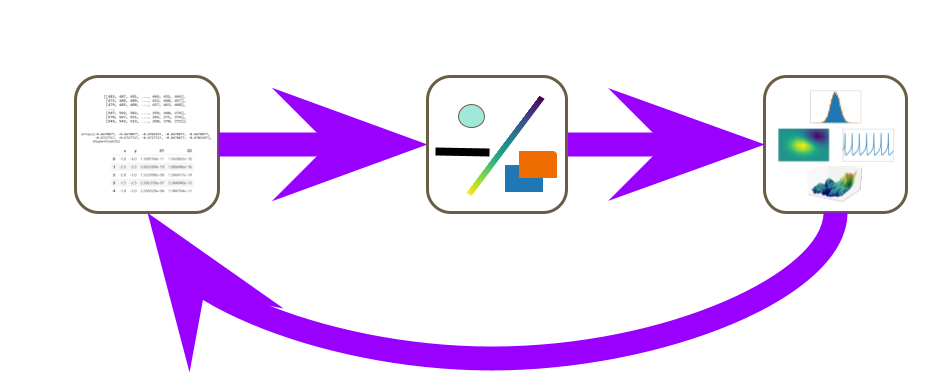
\includegraphics[width=\linewidth]{figures/flow/s2.png}
            \onslide<2|handout:2>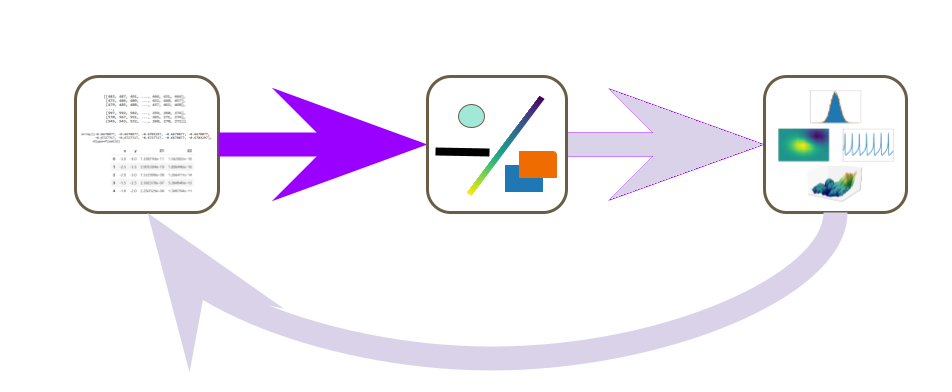
\includegraphics[width=\linewidth]{figures/flow/s_vc.png}
            \onslide<3|handout:3>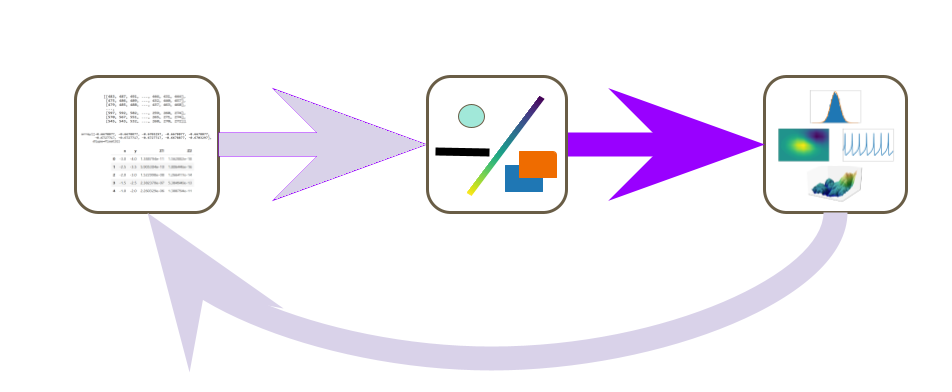
\includegraphics[width=\linewidth]{figures/flow/s_mark.png}
            \onslide<4|handout:4>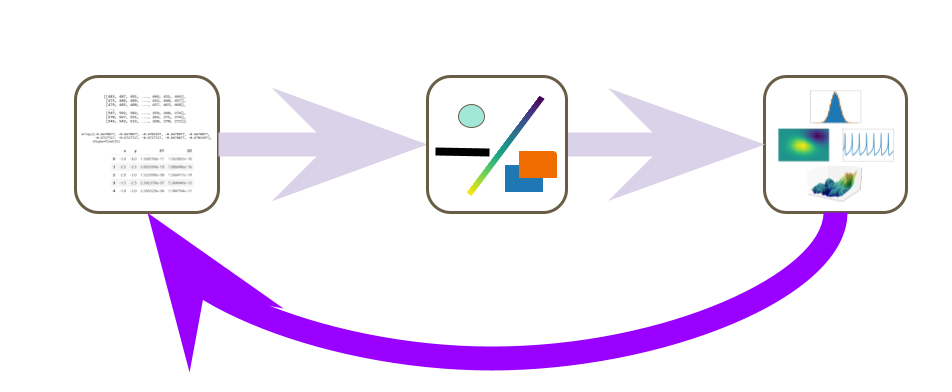
\includegraphics[width=\linewidth]{figures/flow/s3.png}
        \end{overprint}
    \end{figure}
\end{frame}



\begin{frame}{Matplotlib}
    \begin{figure}
       
\includegraphics[width=\linewidth]{figures/flow/artists.png}
    \end{figure}
\end{frame}


\begin{frame}{How do we express structure?}

    \begin{description}
        \item[\textcolor{fiber}{\textbf{field}}]is a set of values of the same type, e.g. one column of a table or the pixels of an image
        \item[\textcolor{base}{\textbf{topology}}] is the connectivity and relative positioning of elements in a dataset \cite{wilkinsonGrammarGraphics2005}.
    \end{description}
\end{frame}

\begin{frame}{Structure Preservation: Equivalent scales and transforms}

\begin{definition}\label{def:related-work:action}\cite{grimaldiDiscreteCombinatorialMathematics2006}
    An \textcolor{action}{\textbf{action}} of \textcolor{action}{$G = (G,\circ, e)$} on $X$ is a function  $act: \textcolor{action}{G} \times X \rightarrow X$. An action has the properties of identity $act(\textcolor{action}{e}, x) = x$ for all  $x \in X$ and associativity $act(\textcolor{action}{g}, act(\textcolor{action}{f}, x)) = act(\textcolor{action}{f} \circ \textcolor{action}{g}, x)$ for $\textcolor{action}{f},\textcolor{action}{g} \in \textcolor{action}{G}$.
\end{definition}
\end{frame}

\begin{frame}{Fields: Equivariance }

    Given a group $G$ that acts on both the input $X$ and the output $Y$ of a function $f: X \rightarrow Y$
    \begin{definition}\label{def:equivariance}
     A function $f$ is \textbf{equivariant} when $f(act(g,x)) = act(g,f(x))$ for all $g$ in $G$ and for all $x$ in $X$ \cite{pittsNominalSetsNames2013}
    \end{definition}
\end{frame}
\begin{frame}{Fields: Equivariance}
    \begin{figure}
        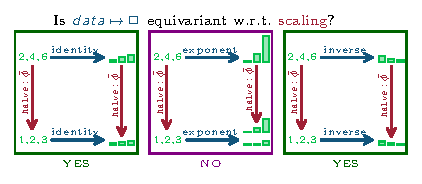
\includegraphics[width=\linewidth]{../paper/figures/equivariant.pdf}
        \label{fig:related-work:equivariance}
      \end{figure}
\end{frame}

\begin{frame}{Fields: Homomorphism}
    Given the function $f: X \rightarrow Y$, with operators $(X, \circ)$ and $(Y, *)$

    \begin{definition}\label{def:homomorphism}
      A function $f$ is \textbf{homomorphic} when $f(x_1 \circ x_2) = f(x_1) * f(x_2)$ and preserves identities $f(I_x) = I_y$ all $x, y \in X$ \cite{grimaldiDiscreteCombinatorialMathematics2006}
    \end{definition}
\end{frame}


\begin{frame}{Fields: Homomorphism}

    \begin{figure}
        \includegraphics[width=\linewidth]{../paper/figures/homomorphism.pdf}
        \label{fig:related-work:homomorphism}
      \end{figure}
\end{frame}


\begin{frame}{Topology: Homeomorphism}

    \begin{definition}
        A function $f$ is a $homeomorphism$ if it is bijective, continuous, and has a continuous inverse function $f^{-1}$.
      \end{definition}
\end{frame}

\begin{frame}{Homeomorphic topology}
    \begin{figure}
        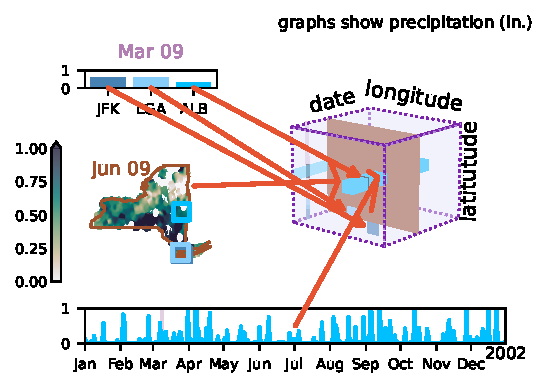
\includegraphics[width=\linewidth]{../paper/figures/k_different_types.pdf}
    \end{figure}
\end{frame}


\begin{frame}{Structure Preservation}
    \begin{itemize}
        \item Bertin: equivalent data and visual field properties \cite{bertinSemiologyGraphicsDiagrams2011}
        \item Mackinlay: homomorphic fields and equivalent topology \cite{mackinlayAutomaticDesignGraphical1987}
        \item Wilkinson: homomorphic scales and  equivalent topology \cite{wilkinsonGrammarGraphics2005}
        \item Kindleman  \& Schieidegger: equivariant scales, invariant data representation, equivalent topology \cite{kindlmannAlgebraicProcessVisualization2014}
    \end{itemize}
    \begin{block}{contribution}
    explicit homeomorphic topology, equivariant actions on fields and topology
    \end{block}
\end{frame}


\begin{frame}{Domain Specific Library: library assumes structure \cite{HeerSoftware2006}}
    \begin{table}
        %\renewcommand{\arraystretch}{2}
        %
        \begin{tabular}{>{\onslide<1->}l>{\onslide<2->}l>{\onslide<3->}l}
            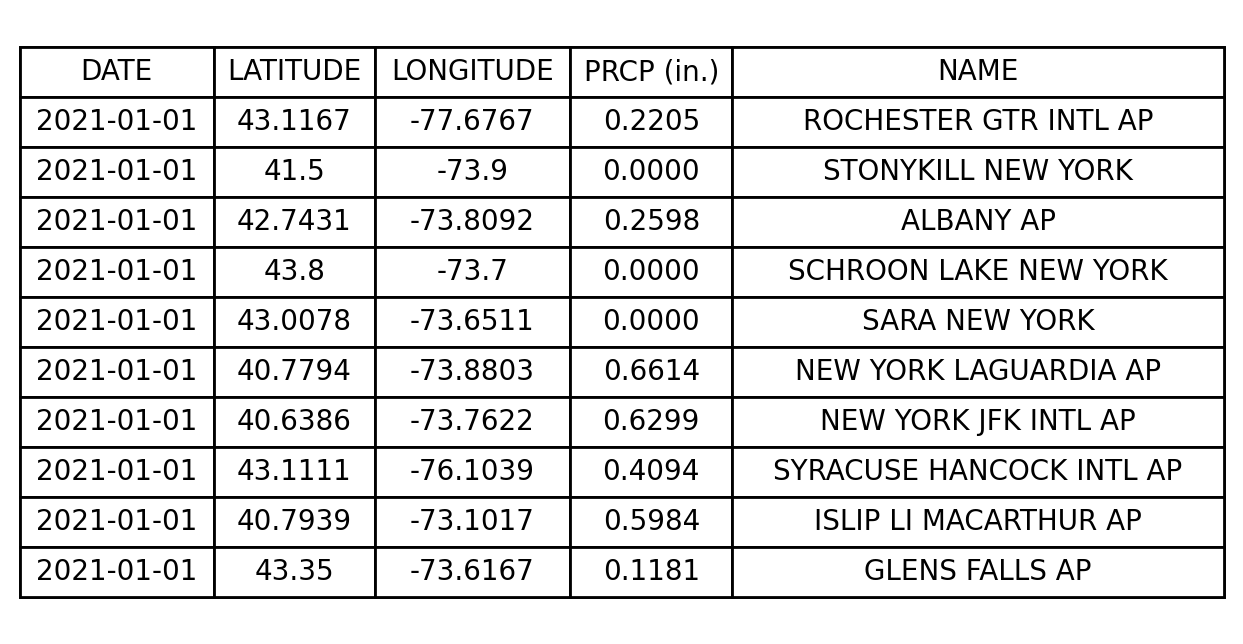
\includegraphics[width=.24\textwidth]{figures/intro/table.png} & 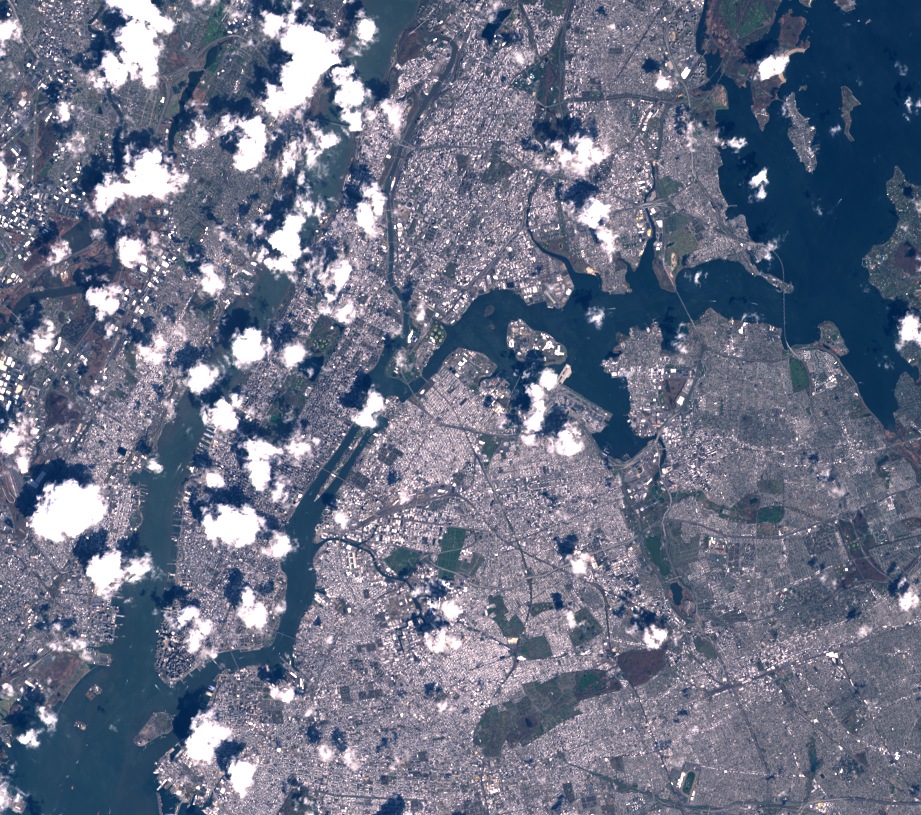
\includegraphics[width=.3\textwidth]{figures/intro/landsat.png} & 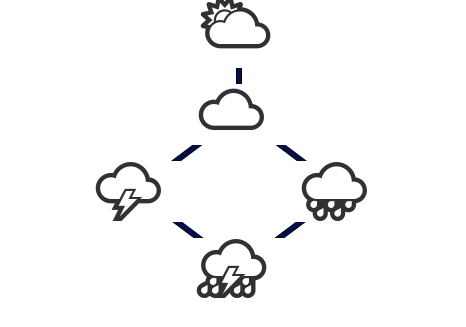
\includegraphics[width=.33\textwidth]{figures/math/graph.png} \\
            ggplot\cite{wickhamGgplot2ElegantGraphics2016}  & ImageJ\cite{schneiderNIHImageImageJ2012}& Gephi\cite{bastianGephiOpenSource2009}\\
            Vega\cite{satyanarayanDeclarativeInteractionDesign2014} & ImagePlot\cite{studiesCulturevisImageplot2021} & Graphviz\cite{ellsonGraphvizOpenSource2002}\\
            Altair\cite{vanderplasAltairInteractiveStatistical2018}& Napari\cite{nicholas_sofroniew_2021_4533308} & Networkx\cite{HagbergExploringNetwork2008}\\
             Tableau \cite{StoltePolaris2002}& &\\
            \cite{hanrahanVizQL2006,MackinlayShowme2007}&&\\
        \end{tabular}
    \end{table}
\end{frame}

\begin{frame}
    \frametitle{Building Block Library\cite{wongsuphasawatNavigatingWideWorld2021}: visual algorithms assume structure \cite{toryRethinkingVisualizationHighlevel2004}}

    \begin{enumerate}
        \item Matplotlib\cite{hunterMatplotlib2DGraphics2007} $\rightarrow$ Seaborn\cite{Waskom2021}, xarray \cite{hoyer2017xarray}
        \item D3 \cite{bostockDataDrivenDocuments2011}
        \item VTK \cite{hanwellVisualizationToolkitVTK2015,geveciVTK2012},MayaVi\cite{RamachandranMayaVI2011}$\rightarrow$ Titan\cite{brianwylieUnifiedToolkitInformation2009}, ParaView\cite{ahrens2005paraview}
    \end{enumerate}
\end{frame}

\section{Algebraic Topology \& Category Theory}
\begin{frame}<presentation:1|handout:1>{Design Composable Structure Preserving API}
    \begin{description}
        \item[Fiber Bundles] Butler: "unified, dimension-independent framework" that expresses data as the mapping between continuity and fields \cite{butlerVectorBundleClassesForm1992,butlerVisualizationModelBased1989}
        \item[Simplicial Databases] Spivak: Add rich typing for fields to Bulter \cite{spivakSimplicialDatabases2009}
        \item[Category Theory Language] express constraints in specifications \cite{wielsManagementEvolvingSpecifications1998}
        \item[Sheaves] Ghrist "algebraic data structure" for representing data over topological spaces \cite{ghristElementaryAppliedTopology2014}
    \end{description}
\end{frame}


\subsection{Uniform Abstraction for Data \& Graphics}

\begin{frame}<presentation:1|handout:1>{Expressive Types}
    \begin{equation*}
        \textcolor{section}{\texttt{dataset}}: \textcolor{base}{\texttt{topology}} \rightarrow \textcolor{fiber}{\texttt{fields}}
      \end{equation*}
\end{frame}

\subsubsection{Abstract data representation}
\begin{frame}{Fiber Bundle}

    \begin{definition}\label{def:fiber_bundle}
       A \textbf{fiber bundle} $(\dtotalc, \dbasec, \pi, \dfiberc)$ is a structure with topological spaces $\dtotalc, \dfiberc, \dbasec$ and  bundle projection map $\pi: \dtotalc \rightarrow \dbasec$ \cite{spanier1989algebraic}.

       \begin{equation} \label{eq:atct:fb:intro}
        \begin{tikzcd}[ampersand replacement=\&]
          \dfiberc \arrow[r, hook, color=total] \& \dtotalc \arrow[r, "\pi", color=total, two heads] \& \dbasec
          \end{tikzcd}
        \end{equation}

    A continuous surjective map $\bm{\pi}$ is a \textbf{bundle projection} map when
    \begin{enumerate}
      \item all fibers in the bundle are isomorphic. Since all fibers are isomorphic $\dfiber \cong \dfiber_{\dbasepoint}$ for all points $\dbasepoint \in \dbase$, there is a uniquely determined \textcolor{fiber}{fiber space} \dfiberc\ given by the preimage of the projection $\pi$ at any point $\dbasepoint$ in the \textcolor{base}{base space} \dbasec: $\dfiberc = \pi^{-1}(k)$.
      \item each point $\dbasepointc$ in the \textcolor{base}{base space} \dbasec\ has an open neighborhood $\openset_{\dbasepointc}$ such that the \textcolor{total}{total space} \dtotalc\ over the neighborhood is locally trivial.
    \end{enumerate}
    \end{definition}

    \textbf{Local triviality} means $\dtotal\vert_{\openset} = \openset\times \dfiber$.
\end{frame}

\begin{frame}{Fiber Bundle}
    \begin{figure}
        \includegraphics[width=\linewidth]{../paper/figures/transition_maps.pdf}
    \end{figure}
\end{frame}

\begin{frame}{Fiber Bundle: section}

    \begin{minipage}{.5\columnwidth}
        \begin{definition}\label{def:fiber_bundle:section}
        A \textcolor{section}{\textbf{section}} $\dsectionc: \dbasec \rightarrow \dtotalc$ over a fiber bundle is a smooth right inverse of $\pi(\dsection(\dbasepoint)) = \dbasepoint$ for all $\dbasepoint \in \dbase$
        \end{definition}
        \end{minipage}
        \begin{minipage}{.4\columnwidth}
          \begin{equation} \label{eq:atct:fb:intro-sec}
            \begin{tikzcd}[ampersand replacement=\&, row sep=huge]
             \dfiberc
              \arrow[r, hook, color=total] \&
              \dtotalc
              \arrow[d, "\pi"',color=total, two heads] \\
               \&
            \dbasec
               \arrow[u, "\dsectionc"', bend right, pos=.5, color=section, dashed]
            \end{tikzcd}
          \end{equation}
        \end{minipage}
\end{frame}

\begin{frame}{Fiber Bundle: section}
    \begin{figure}
        \includegraphics[width=\textwidth]{../paper/figures/fb.pdf}
    \end{figure}
\end{frame}

\subsubsection{Topology: base Space \dbasec}

\begin{frame}{Base space: topology}
The base space of a fiber bundle is a quotient topology\cite{munkresElementsAlgebraicTopology1984}. Given a set $X$ and a function $\mathcal{N}:X\to 2^{2^X}$ that assigns to any $x\in X$ a non-empty collection of subsets $\mathcal{N}(x)$, where each element of $\mathcal{N}(x)$ is a \emph{neighborhood of $x$}, then $X$ with  $\mathcal{N}$ is a \textcolor{base}{topological space} and $\mathcal{N}$ is a neighborhood \emph{topology} if for each $x$ in $X$: \cite{brownronaldTopologyGroupoids2006}

\begin{definition}\label{def:topology}
\begin{enumerate}
  \item if $N$ is a neighborhood $N \in \mathcal{N}(x)$ of $x$ then $x \in N$
  \item every superset of a neighborhood of $x$ is a neighborhood of $x$; therefore a union of a neighborhood and adjacent points in $X$ is also a neighborhood of $x$
  \item the intersection of any two neighborhoods of $x$ is a neighborhood of $x$
  \item any neighborhood $N$ of $x$ contains a neighborhood $M \subset N$ of $x$ such that $N$ is a neighborhood of each of the points in $M$
\end{enumerate}
\end{definition}
\end{frame}

\begin{frame}{Why neighborhood topology?}
\begin{figure}
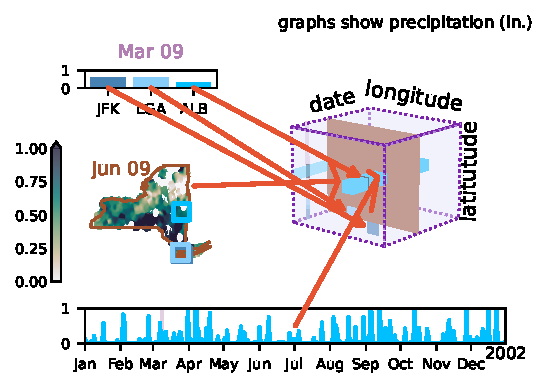
\includegraphics[width=\linewidth]{../paper/figures/k_different_types.pdf}
\end{figure}
\end{frame}

\begin{frame}{Base \texttt{TYPE} \dbasec}
    \begin{definition}\label{def:atct:category}
        An \textbf{category} $\mathcal{C}$ consists of the following \textit{data}:
     \begin{enumerate}
       \item a collection of \textit{objects} $X \in \textbf{ob}(\mathcal{C})$
       \item for every pair of objects $X, Y \in \textbf{ob}(\mathcal{C})$, a set of \textit{morphisms} $X \xrightarrow{f} Y \in Hom_{\mathcal{C}}(X, Y)$
       \item for every object $X$, a distinct \textit{identity morphism} $X \xrightarrow {id_x} X$ in $Hom_{\mathcal{C}}(X, X)$
       \item a \textit{composition function} $f \in Hom_{\mathcal{C}}(X, Y) \times  g \in Hom_{\mathcal{C}}(Y, Z) \rightarrow g \circ f \in Hom_{\mathcal{C}}(X, Z)$
     \end{enumerate}
     such that
     \begin{enumerate}
       \item \textit{unitality:} for every morphism $ X \xrightarrow{f} Y$, $f \circ id_x = f = id_y \circ f$
       \item \textit{associativity:} if any three morphisms $f, g, h$ are composable,
         \begin{equation*}
           \begin{tikzcd}[ampersand replacement=\&]
             X \arrow[r, "f"] \arrow[rrr, "h\circ(g\circ f) = (h\circ g)\circ f"', bend right, dashed] \& Y  \arrow[r, "g"] \& Z \arrow[r, "h"] \& W
             \end{tikzcd}
       \end{equation*}
       then they are associative such that $h\circ(g\circ f) = (h \circ g) \circ f$  \cite{lawvere2009conceptual,riehlCategoryTheoryContext,maclaneCategoriesWorkingMathematician2013,fongInvitationAppliedCategory2019}.
       \end{enumerate}
     \end{definition}
\end{frame}

\begin{frame}{Add records $\rightarrow$ Add to base space}
    \begin{figure}
        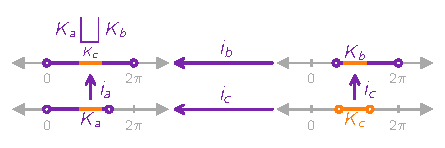
\includegraphics[width=\textwidth]{../paper/figures/tex/k_coproduct.pdf}
    \end{figure}
\end{frame}

\subsubsection{fields: fiber space \dfiberc}

\begin{frame}{Field types }
   A \textit{schema} consists of a pair $(\fnames, \sigma)$ where $\fnames$ is the set of field names and $\sigma: \fnames \rightarrow \textbf{DT}$ is a function from field name to field data type\cite{spivakSimplicialDatabases2009}

   The function $\sigma$ is composed with $\pi$ such that $\pi^{-1}(\sigma(C)) \subseteq \mathscr{U}$; this composition induces a domain bundle $\pi_{\sigma}:\mathscr{U}_{\sigma} \rightarrow \fnames$ that associates a field name $c \in C$ with its corresponding domain $\pi^{-1}_{\sigma}(C) \subseteq \mathscr{U}_{\sigma}$.

\end{frame}

\begin{frame}{Record}
    \begin{definition} A \textbf{record} is a function $\delement: \fnames \rightarrow \mathscr{U}_{\sigma}$ and the set of records on $\pi_{\sigma}$ is denoted $\Gamma^{\pi}(\sigma)$. Records must return an object of type $\sigma(\fname) \in \textbf{DT}$ for each field $c \in C$.
    \end{definition}

    Tables are sections $\dsection: \dbase \rightarrow \Gamma^{\pi}(\sigma)$ from an indexing space $\dbase$ to the set of all possible records $\Gamma^{\pi}(\sigma)$ on the schema bundle
\end{frame}

\begin{frame}{Fiber \texttt{TYPE} \dfiberc}
    We define the \textcolor{fiber}{fiber space} \dfiberc\ to be the space of all possible data records
    \begin{equation}
      \dfiberc \coloneqq \{\delement: \fnames \rightarrow \mathscr{U}_{\sigma} \bigm{\vert} \pi_{\sigma}(\delement(\fname)) = \fname\;for\;all\; \fname \in \fnames \}
    \end{equation}
    such that the preimage of a point is the corresponding data type domain $\pi^{-1}(\dbasepoint) = \dfiber_{k} = \mathscr{U}_{{\sigma}_{\dbasepoint}}$.
\end{frame}

\begin{frame}{Fiber category \dfiberc}
    The fiber category has a single object $\dfiberc$ of an arbitrary type and morphisms on the fiber object $\dfunctc \in Hom(\dfiberc, \dfiberc)$.

    The fiber category $\mathcal{\dfiberc}$ is also equipped with a bifunctor  $\otimes: \mathcal{\dfiber} \times \mathcal{\dfiber} \rightarrow \mathcal{\dfiber}$ for combining fiber types.
\end{frame}

\begin{frame}{Fiber morphism \dfunctc}
    \begin{table}
        \begin{tabular}{|lll|}\hline
            scale & operators & sample constraint \\ \hline
            nominal & $=,\neq$ &  $\dsectionc(\dbasepointc_1) \neq \dsectionc(\dbasepointc_2)\implies \dfunctc (\dsectionc(\dbasepointc_1)) \neq\dfunctc(\dsectionc(\dbasepointc_2))$\\
            ordinal & $<, \leq, \geq, >$ &  $\dsectionc(\dbasepointc_1) \leq \dsectionc(\dbasepointc_2) \implies \dfunctc (\dsectionc(\dbasepointc_1)) \leq \dfunctc(\dsectionc(\dbasepointc_2)$) \\
            interval & $+, -$ &  $\dfunctc(\dsectionc(\dbasepointc) + C) = \dfunctc(\dsectionc(\dbasepointc)) + C$ \\
            ratio & $*,/$ &  $\dfunctc(\dsectionc(\dbasepointc) * C) = \dfunctc(\dsectionc(\dbasepointc))*C $\\ \hline
        \end{tabular}
    \end{table}

\end{frame}

\begin{frame}{Constraints as definition: Dates}
    \begin{itemize}
        \item year:  $\{y \in \mathbb{I}\vert 1992 \leq y \leq 2025\}$
        \item month:  $\{m \in \mathbb{I}\vert 1 \leq m \leq 12 \}$
        \item day: $\{d \in \mathbb{I}\vert 1 \leq d \leq 31 \}$
        \item date:  $ \otimes: \dfiber_{year} \times \dfiber_{month} \times \dfiber_{day} \rightarrow \dfiber_{date}$
    \end{itemize}
    where the composition $\otimes$ includes the constrain to only return dates that have the right number of days for each month.
\end{frame}

\begin{frame}{Expand records $\rightarrow$ multiply fiber space}

    \begin{figure}
        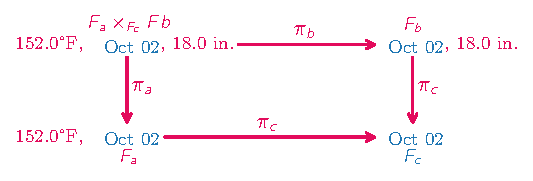
\includegraphics[width=\textwidth]{../paper/figures/tex/f_product.pdf}
    \end{figure}
\end{frame}

\subsubsection{Dataset: section}

\begin{frame}{local sections}
    We define section functions locally:
    \begin{equation}
      \label{eq:atct:fb:sections}
      \cgamma{\opensetc}{\dtotalc\restriction_{\opensetc}} \coloneqq \big\{\dsectionc: \opensetc\rightarrow \dtotalc\restriction_{\opensetc} \; \bigm{\vert} \pi(\dsectionc(\dbasepointc)) = \dbasepointc\;for\, all\; \dbasepointc \in \opensetc \big\}
    \end{equation}
    such that each section function $\dsection: \dbasepoint \mapsto \delement$ maps from each point $\dbasepoint \in \openset$ to a corresponding record in the fiber space $\delement \in \dfiber_{\dbasepoint}$ over that point.

    This encoding can be translated into a set of signatures $\{\textcolor{section}{\texttt{data-subset}}: \textcolor{base}{\texttt{topology}} \rightarrow \textcolor{fiber}{\texttt{fields}}$ s.t. $\textcolor{section}{\texttt{data-subset}} \subset \textcolor{section}{\texttt{dataset}}\}$.
\end{frame}

\begin{frame}{global sections}
    When a bundle is trivial $\dtotalc = \dbasec \times \dfiberc$, we can defined a global sections $\dsection: \dbase \rightarrow \dfiber \in \Gamma(\dbase, \dfiber)$ which we translate into a data signature of the form $\textcolor{section}{\texttt{dataset}}: \textcolor{base}{\texttt{topology}} \rightarrow \textcolor{fiber}{\texttt{field}}$ where $\dsectionc=\textcolor{section}{\texttt{dataset}}$, $\dbasec=\textcolor{base}{\texttt{topology}}$ and $\dfiberc=\textcolor{fiber}{\texttt{fields}}$
\end{frame}

\begin{frame}{Graphic bundle and section}
    \begin{equation}
        \label{eq:atct:fb:graphic}
        \begin{tikzcd}[ampersand replacement=\&]
            \gfiberc \arrow[r, hook, color=total] \& \gtotalc \arrow[r, "\pi", two heads, color=total] \& \gbasec
        \end{tikzcd}
    \end{equation}

    \begin{equation}\label{eq:atct:fb_graphic_section}
        \begin{split}
        \cgamma{\opensetgc}{\gtotalc\restriction_{\opensetgc}} & \coloneqq \\
        &\big\{\gsectionc: \opensetgc\rightarrow \gtotalc\restriction_{\opensetgc} \; \bigm{\vert} \pi(\gsectionc(\gbasepointc)) = \gbasepointc\;for\, all\; \gbasepointc \in \opensetgc \big\}
        \end{split}
      \end{equation}
\end{frame}

\begin{frame}{Graphic section}
\begin{figure}
    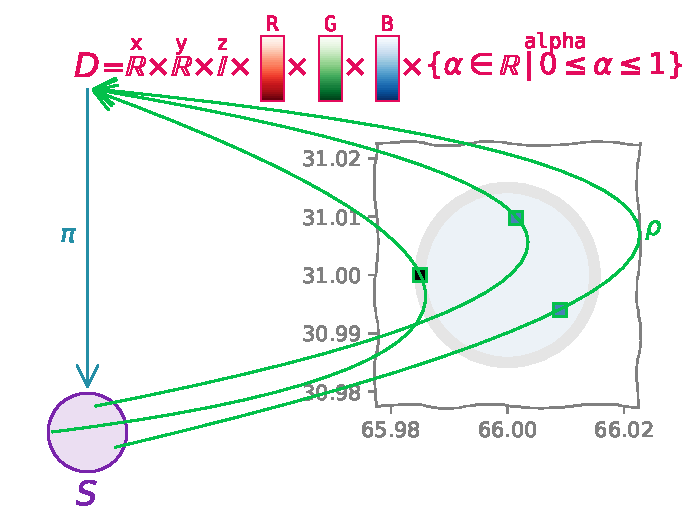
\includegraphics[width=\linewidth]{../paper/figures/fb_rho.pdf}
\end{figure}
\end{frame}

\subsection{Abstract Data Containers}

\begin{frame}{functors}
    \begin{definition}\cite{bradleyWhatFunctorDefinitions,bradleyTopologyCategoricalApproach2020} A \textbf{functor} is a map $F: \mathcal{C} \rightarrow \mathcal{D}$, which means it is a function between objects $F: \textbf{ob}(\mathcal{C}) \mapsto \textbf{ob}(\mathcal{D})$ and that for every morphism $f \in Hom(C_1, C_2)$  there is a corresponding function $F: Hom(C1, C2) \mapsto Hom(F(C_1), F( C_2))$.
        A \textbf{functor} must satisfy the properties
        \begin{itemize}
          \item \textit{identity}: $F(id_{C}(C)) = id_{D}(F(C))$
          \item \textit{composition}: $F(g)\circ F(f) = F(g\circ f)$ for any composable morphisms $C_{1}\xrightarrow{f} C_2$, $C_2 \xrightarrow{g} C_3$
        \end{itemize}
        $F(C) \in \textbf{ob}(\mathcal{D})$ denotes the object to which an object $C$ is mapped, and $F(f) \in Hom(F_(C_1), F_(C_2))$ denotes the morphism that $f$ is mapped to.
        \end{definition}
\end{frame}

\begin{frame}{topological equivariance: presheaf}
    \begin{definition}\label{def:atct:presheaf}
        A \textbf{presheaf} $F:\mathcal{C}^{op} \rightarrow \setb$ is a contravariant functor from an object in an arbitrary category to an object in the category \setb\cite{spanier1989algebraic}.
    \end{definition}
    The presheaf is contravariant when for every arbitrary morphism between input base spaces $\dfunch: \openset_1 \rightarrow \openset_2$ there exists a corresponding pullback function between the sets of sections $\dfuncpull: \cgamma{\opensetc_2}{\dtotalc\restriction_{\opensetc_2}} \rightarrow \cgamma{\opensetc_1}{\dtotalc\restriction_{\openset_c1}}$.
\end{frame}

\begin{frame}{topological equivariance: presheaf}
    \begin{figure}
        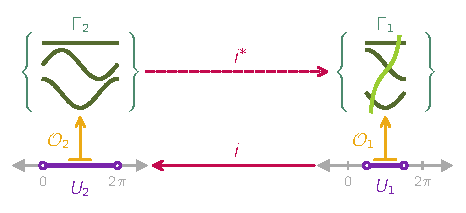
\includegraphics[width=\textwidth]{../paper/figures/tex/presheaf.pdf}
    \end{figure}
\end{frame}

\begin{frame}{Container invariance: sheaf}
    \begin{definition}\label{def:atct:sheaf}\cite{bakerEuclideanSpaceMathsSheaf,spanier1989algebraic} A \textbf{sheaf} is a presheaf that satisfies the following two axioms
        \begin{itemize}
          \item \textit{locality} two sections in a sheaf are equal $\dsection^{a} = \dsection^{b}$ when they evaluate to the same values $\dsection^{a}\vert_{\openset_i} =  \dsection^{b}\vert_{\openset_i}$ over the open cover $\bigcup_{i\in I} \openset_{i} \subset \openset$ (indexed by $I$).
          \item \textit{gluing} the union of sections defined over subspaces $\dsection^{i} \in \Gamma(\openset_i, \dtotal|_{\openset_i})$ is equivalent to a section defined over the whole space $\dsection\vert_{\openset_i} = \dsection^{i}$ for all $i\in I$ if all pairs of sections agree on overlaps $\dsection^{i}\vert_{\openset_i\cap\openset_j} =  \dsection^{j}\vert_{\openset_i\cap\openset_j}$
          \end{itemize}
        \end{definition}
\end{frame}

\begin{frame}{Container invariance: sheaf}
\begin{figure}
    \includegraphics[width=\linewidth]{../paper/figures/tex/sheaf_rules.pdf}
\end{figure}
\end{frame}

\begin{frame}{What about needing more than one record?}
    The sheaf over a very small region surrounding a point $\dbasepoint$ is called a \textit{stalk}\cite{harder2008lectures}
\begin{equation}
  \label{eq:atct:sheaf:stalk}
    \sheaf_{\dbase, \dtotalc}\restriction_{\dbasepoint}\coloneqq \lim\limits_{\openset\ni \dbasepoint} \Gamma(\openset, \dtotal\restriction_{\openset})
\end{equation}
where the fiber is contained inside the stalk  $\dfiber_{\dbasepoint} \subset  \sheaf_{\dbase, \dtotal}\restriction_{\dbasepoint}$. The \textit{germ} is the section evaluated at a point in the stalk  $\dsection(\dbasepoint) \in \sheaf_{\dbase, \dtotal}\restriction_{\dbasepoint}$ and is the data.
\end{frame}
\section{Artist}

\subsection{Homeomorphism}
\begin{frame}{Homeomorphism}
    We define the mapping \vindexc\ to be a surjective continuous map:
    \begin{equation}
      \label{eq:atct:xi}
      \vindexc: \opensetgc \textcolor{functor}{\rightarrow} \opensetc
    \end{equation}
    between a graphic subspace $\opensetg \subseteq \gbase$ and data subspace $\openset \subseteq \dbase$.

    The set of points in graphic space that correspond to each point in data space is
\begin{equation}
  \label{eq:atct:xi:inverse}
  \vindexprec(\dbasepointc) = \{\gbasepointc | \vindexc(\gbasepointc) = \dbasepointc \forall \dbasepointc \in \dbase, \gbasepointc \in \gbasec\}
\end{equation}
such that every point in a graphic space has a corresponding point in data space.
\end{frame}

\begin{frame}{Homeomorphism}
    \begin{figure}
        \includegraphics[width=\textwidth]{../paper/figures/xi_zoom.pdf}
    \end{figure}
\end{frame}

\begin{frame}{Pushforward: Graphic for Data}
    \begin{definition} Given a sheaf $\sheaf_{\gbase, \gtotal}$ on $\gbase$, the \textbf{pushforward} sheaf  $\vindexpush\sheaf_{\gbase, \gtotal}$ on $\dbase$ is defined as
        \begin{equation}
          \vindexpushc(\sheafc_{\gbasec, \gtotalc})(\opensetc)  = \sheafc_{\gbasec, \gtotalc}(\vindexc^{-1}(\opensetc))
        \end{equation}
      for all opensets $\opensetc \subset \dbasec$\cite{harder2008lectures}.
    \end{definition}
This provides a way to look up which graphic corresponds with a data index
\begin{equation}
  \label{eq:atct:sheaf:pushforward_select}
  \vindexpushc\gsectionc(\dbasepointc) = \gsectionc\restriction_{\vindexprec(\dbasepointc)}
\end{equation}
such that $\vindexpush\gsection(\dbasepoint))(\gbasepoint) = \gsection(\gbasepoint)$ for all $\gbasepoint \in \vindexpre(\dbasepoint)$.
\end{frame}

\begin{frame}{Pullback: Data at graphic }
    \begin{definition} \cite{harder2008lectures} Given a sheaf $\sheaf_{\dbase, \dtotal}$ on $\dbase$, the \textbf{pullback} sheaf $\vindexpullc\sheafc_{\dbasec, \dtotalc}$ on $\gbasec$ is defined as the sheaf associated to the presheaf $\vindexpullc(\sheafc_{\dbasec, \dtotalc})(\opensetgc) = \sheafc_{\dbasec, \dtotalc}(\vindexc(\opensetgc))$ for $\vindex(\opensetgc) \in \dbase$.
    \end{definition}

    This provides a way to then look up what data values correspond with a graphic index
    \begin{equation}
      \label{eq:atct:sheaf:pullback_hover}
      \vindexpullc\dsectionc(\gbasepointc) = \dsectionc(\vindexc(\gbasepointc)) = \dsectionc(\dbasepointc)
    \end{equation}
    As \vindex\ is surjective, there are many points $\gbasepoint \in \opensetg\subseteq\gbase$ in the graphic space that correspond to a single point $\vindex(\gbasepoint) = \dbasepoint$.
\end{frame}

\begin{frame}{Homeomorphism}
    \begin{figure}
        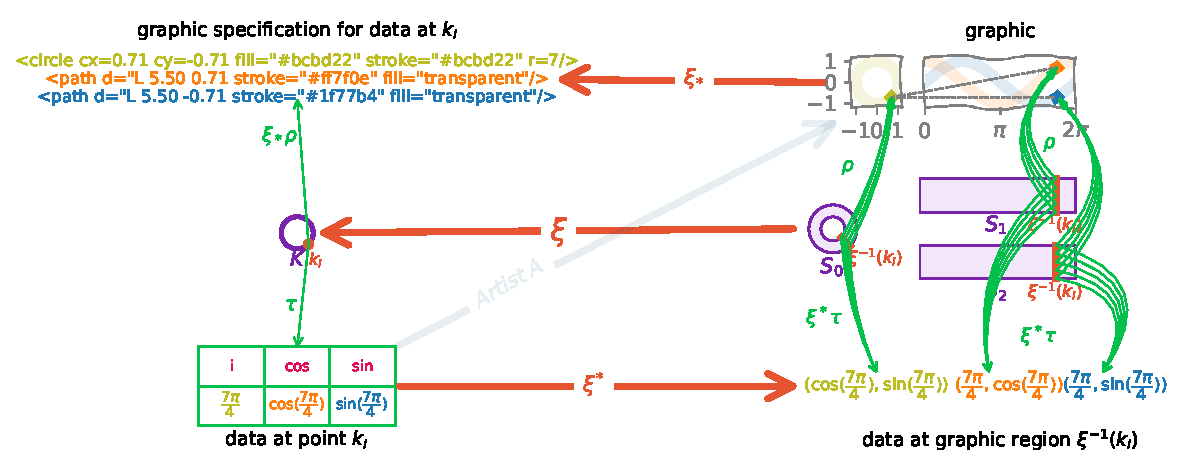
\includegraphics[width=\textwidth]{../paper/figures/xi_diagram.pdf}
    \end{figure}
\end{frame}

\begin{frame}{Artist}
    \begin{definition}\label{def:natural-transform}
        Given two functors $F, G: \mathcal{C}\rightarrow \mathcal{D}$, a \textbf{natural transformation} $\alpha: F \rightarrow G$ is a function which assigns to each object $c$ of $\mathcal{C}$ a morphism $\alpha_c:F(input) \rightarrow G(c), G(c) \in \mathcal{D}$, in such a way that for every morphism $f:c \rightarrow c^\prime, c^\prime \in \mathcal{C}$, the morphisms in $\mathcal{D}$ commute such that $\alpha_c^{\prime}(F(f)(F(c))) = G(f)(\alpha_c(F(c))$. When this holds, $\alpha_{c}$ is \textit{natural} in $c$.\cite{maclaneCategoriesWorkingMathematician2013}.
      \end{definition}

\end{frame}


\begin{frame}{Artist}

\begin{equation*}
    \begin{tikzcd}[ampersand replacement=\&]
      \& {} \arrow[dd, "\texttt{artist}" description, Rightarrow, shift left=3.65, shorten <= .7em, shorten >= .7em, color=artist, font=\Huge]
      \& \\ {\scriptstyle\textcolor{base}{\texttt{topology}}}
        \arrow[rr, "\texttt{graphic}"', bend right, color=sheaf, font=\huge] \arrow[rr, "\texttt{data}", bend left, color=sheaf, font=\huge] \&
      \& {\scriptstyle\textcolor{base}{\texttt{topology}}\textcolor{section}{\rightarrow} \textcolor{fiber}{\texttt{fields}}} \\
      \& {}                                              \&
  \end{tikzcd}
  \end{equation*}
\end{frame}

\begin{frame}{How?}
    \begin{equation}
        \label{eq:artist:homset}
        \begin{tikzcd}[ampersand replacement=\&, column sep=50]
       \cgamma{\opensetc}{\vindexpushc\gtotalc\restriction_{\opensetc}}
      \& \cgamma{\opensetgc},{\gtotalc\restriction_{\opensetgc}}
      \arrow[l, "\vindexpushc"', color=functor]                                          \\
      \cgamma{\opensetc}{\dtotalc\restriction_{\opensetc}}
      \arrow[r, "\vindexpullc", color=functor]
      \arrow[u, "\textcolor{set}{Hom}_{\sheafc_{\dbasec}}", color=homset]
      \arrow[ru, "{\textcolor{set}{Hom}_{\sheafc_{\dbasec},\sheafc_{\gbasec}}}", color=homset]
      \&
      \cgamma{\opensetgc}{\vindexpullc\dtotalc\restriction_{\opensetgc}}
      \arrow[u, "\textcolor{set}{Hom}_{\sheafc_{\gbasec}}"', color=homset]
      \end{tikzcd}
      \end{equation}
\end{frame}

\begin{frame}{Artist}
    \begin{align}
        \label{eq:artist:hom_transport}
        \vartistc:& \cgamma{\dbasec}{\dtotalc}\textcolor{artist}{\rightarrow} \imartist{\gbasec}{\gtotalc}, \imartist{\gbasec}{\gtotalc} \subset \cgamma{\gbasec}{\gtotalc}
      \end{align}
      where:
    \begin{equation}
        \label{eq:artist:output}
        \imartist{\gbasec}{\gtotalc} \coloneqq\\
        \{\gsectionc \mid\;\exists\;\dsectionc \in \cgamma{\dbasec}{\dtotalc}\;s.t.\;
        \vartistc(\dsectionc) = \gsectionc,\; \vindexc(\gbasec) = \dbasec \}
      \end{equation}
\end{frame}

\begin{frame}{Equivariant Artist}
    \begin{equation}
        \label{eq:artist:equivariance}
        \begin{tikzcd}[ampersand replacement=\&, column sep=small]
        \cgamma{\dbasec}{\dtotalc}
        \arrow[rrr, "\vartistc", color=artist]
        \arrow[d, "\dfuncpullc_{\dtotalc}"', color=action]
        \& \& \&
        \imartist{\gbasec}{\gtotalc}
        \arrow[d, "\dfuncpullc_{\gtotalc}", dotted] \\
        \cgamma{\dbasec^{\prime}}{\dfuncpullc_{\dtotalc}\dtotalc}
        \arrow[dd, "\dfunctc_{\dtotalc}"', color=action] \&
        \dbasec
         \&
        \gbasec
        \arrow[l, "\vindexc"', color=functor]
        \&
        \imartist{\gbase^{\prime}}{\dfuncpullc_{\gtotalc}\gtotalc}
        \arrow[dd, "\dfunctc_{\gtotalc}", dotted, color=action] \\
        \&
        \dbasec^{\prime}
        \arrow[u, "\dfunchc_{\dtotalc}", color=action]
        \&
        \gbasec^{\prime}
        \arrow[l, "\vindexc"', color=functor]
        \arrow[u, "\dfunchc_{\gtotalc}"', dotted, color=action]
        \& \\
        \cgamma{\dbasec^{\prime}}{\dtotalc^{\prime}}
        \arrow[rrr, "\vartistc", color=artist]
        \& \& \&
        \imartist{\gbasec^{\prime}}{\gtotalc^{\prime}}
        \end{tikzcd}
      \end{equation}
\end{frame}

\begin{frame}{Equivariant Artist}
\begin{figure}
    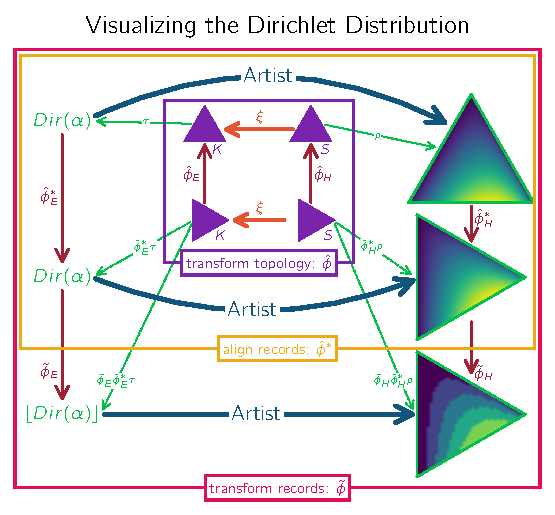
\includegraphics[width=\linewidth]{../paper/figures/artist_equiv.png}
\end{figure}
\end{frame}

\begin{frame}{artist composition}
    \begin{figure}
        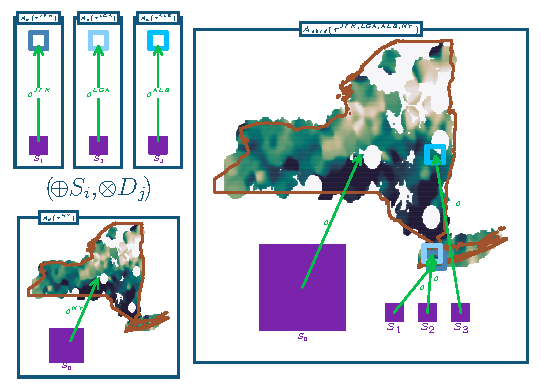
\includegraphics[width=\linewidth]{../paper/figures/composition.pdf}
    \end{figure}
\end{frame}

\begin{frame}{Animation and Interactivity}
    \begin{description}
        \item[pan, zoom, scroll] sheaf: locality + gluing \autoref{def:atct:sheaf}
        \item[selection and hover] pushforward \autoref{eq:atct:sheaf:pushforward_select},  pullback \autoref{eq:atct:sheaf:pullback_hover}
        \item[brushing, linking, annotation] composition of artists \autoref{eq:artist:join_base_fiber}
      \end{description}
\end{frame}

\begin{frame}<presentation:1|handout:1>{Testing if \vartistc\ is equivariant}
    $M$ is a (scaler, vector) measurable component (e.g. color, position, shape, texture, rotation, ) of the rendered visual element.
    \begin{equation*}
    \begin{tikzcd}[ampersand replacement=\&]
    \cgamma{\opensetc}{\dtotalc\restriction_{\opensetc}}
    \arrow[rr, "\vartistc", color=artist]
    \arrow[dd, "\equivc"', color=monoid] \&  \&
    \imartist{\opensetgc}{\gtotalc\restriction_{\opensetgc}}
    \arrow[rr, "render"]
    \arrow[dd, "\extractm", color=monoid]
    \&  \&
    visualization
    \arrow[lldd, "measure"] \\
    \& \& \& \&  \\
    {Hom(\opensetc, \measurec)}
    \arrow[rr, "\vindexpullc"', color=functor]
    \&  \&
    {Hom(\opensetgc,\measurec )}
    \& \&
    \end{tikzcd}
    \end{equation*}
    \begin{description}
        \item[input]{$\equivc: \dsectionc \mapsto (\opensetc \xrightarrow{\equivc_{\dsectionc}} \measurec)$}
        \item[output]{$\extractmc:\gsectionc \mapsto (\opensetgc \xrightarrow{\extractmc_{\gsectionc}} \measurec)$}
        \item[] $\equivc_{\dsectionc}(\dbasepointc) = \extractmc_{\gsectionc}(\gbasepointc)$ for all $\vindexc(\gbasepointc) = \dbasepointc, \dbasepointc \in \dbasec, \gbasepointc \in \gbasec$
    \end{description}
\end{frame}

\section{Construction}
\begin{frame}{Visual Space: Specialized data space}
    $\vfiberc \hookrightarrow \vtotalc \xrightarrow{\pi}\dbasec$
    \begin{figure}
        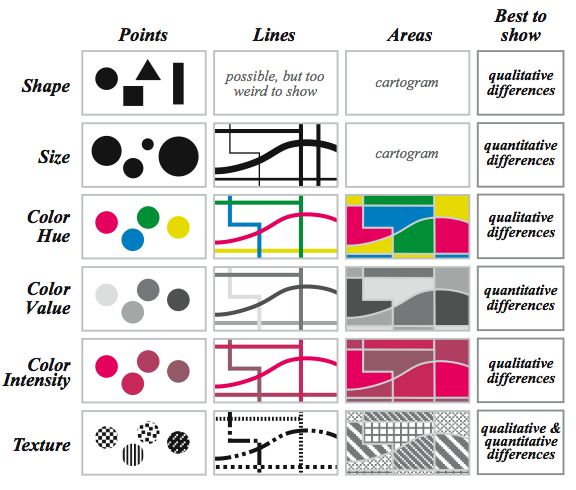
\includegraphics[width=\textwidth]{figures/intro/retinal_variables.png}
    \end{figure}
\end{frame}


\begin{frame}{Encoding}
    \begin{equation}
        \label{eq:constrution:nu}
        \vchannelc: \dfiberc_{\dbasepointc} \rightarrow \vfiberc_{\dbasepoint}
      \end{equation}

      \begin{equation}
        \label{eq:construction:nu:fabrication}
        \begin{tikzcd}[ampersand replacement=\&]
          \dfiberc_{\dbasepointc}
          \arrow[rr, "\vchannelc", color=artist]
          \arrow[rrrr, "\vchannelc^{\prime\prime}", dashed, bend right, color=artist] \&  \&
          \vfiberc_{\dbasepointc}\coloneqq{\dfiberc_{\dbasepointc}^{\prime}}
          \arrow[rr, "\vchannelc^{\prime}", color=artist] \&  \&
          \vfiberc^{\prime}_{\dbasepointc}
        \end{tikzcd}
      \end{equation}
\end{frame}

\begin{frame}{Composition}
    \begin{equation}
        \vmarkc: \cgamma{\dbasec}{\vtotalc} \rightarrow \cgamma{\gbasec}{\gtotalc}
      \end{equation}

      \begin{equation}
        \label{eq:construction:q:fabrication}
        \begin{tikzcd}[ampersand replacement=\&]
            \cgamma{\dbasec}{\vtotalc}
            \arrow[rr, "\vchannel", color=artist]
            \arrow[rrrr, "\vmarkc^{\prime}", bend right, color=artist, dashed] \&  \&
            \cgamma{\dbasec}{\vtotalc^{\prime}}
            \arrow[rr, "\vmarkc", color=artist] \&  \& \cgamma{\gbasec}{\gtotalc}
            \end{tikzcd}
      \end{equation}
\end{frame}

\begin{frame}{Construction Stages}
    \begin{figure}
        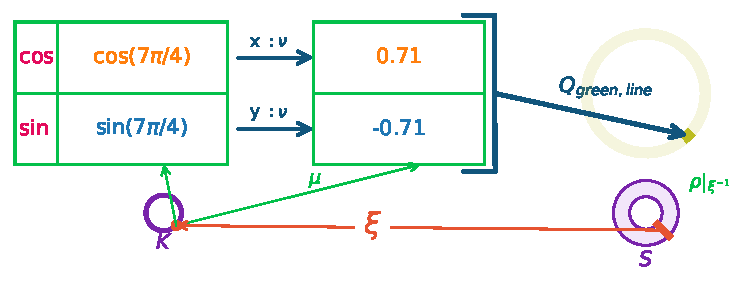
\includegraphics[width=\linewidth]{../paper/figures/construction_nocomp.pdf}
    \end{figure}
\end{frame}


\begin{frame}{Construction Stages: composition}
    \begin{figure}
        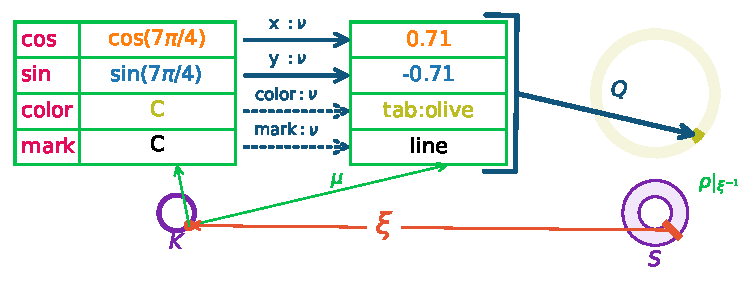
\includegraphics[width=\linewidth]{../paper/figures/construction_comp.pdf}
    \end{figure}
\end{frame}

\begin{frame}{Verify encoder}
    \begin{equation}
        \label{eq:construction:nu:validate}
        \begin{tikzcd}[ampersand replacement = \&, column sep=4em]
          {\dfiberc_{\dbasepointc}^{a}} \times {\dfiberc_{\dbasepointc}^{b}}
          \arrow[d, "\pi_a"', color=fiber]
          \arrow[r, "\vchannelc_{ab}", color=artist]
          \arrow[rr, "\equivc_{ab}", bend left, color=monoid]  \&
          {\vfiberc_{\dbasepointc}^{a}} \times {\vfiberc_{\dbasepointc}^{b}}
          \arrow[d, "\pi_a", color=fiber] \&
          \measurec_{\dbasepointc}^{ab}
          \arrow[d, "\measurec\restriction_a", color=set] \\
          \dfiberc_{\dbasepointc}^a
          \arrow[r, "\vchannelc_{a}", dashed, color=artist] \&
          \vfiberc_{\dbasepointc}^a
          \arrow[r, "\simeq", dotted]  \&
          \measurec_{\dbasepointc}^a   \\
          {\dfiberc_{\dbasepointc}^{a}} \times {\dfiberc_{\dbasepointc}^{c}}
          \arrow[u, "\pi_a", color=fiber]
          \arrow[r, "\vchannelc_{ac}", color=artist]
          \arrow[rr, "\equivc_{ac}", bend right, color=monoid] \&
          {\vfiberc_{\dbasepointc}^{a}} \times {\vfiberc_{\dbasepointc}^{c}}
          \arrow[u, "\pi_a"', color=fiber] \&
          \measurec_{\dbasepointc}^{ac}
          \arrow[u, "\measurec\restriction_a"', color=set]
          \end{tikzcd}
      \end{equation}
\end{frame}
\begin{frame}{Verify encoder}
    \begin{figure}
        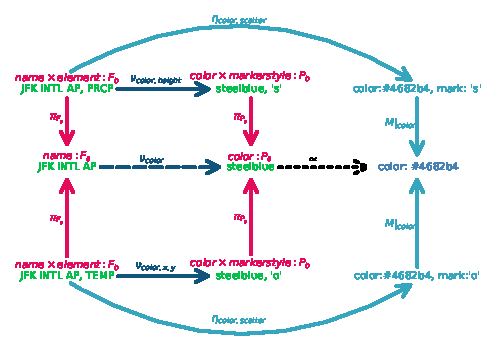
\includegraphics[width=\linewidth]{../paper/figures/encoder.pdf}
    \end{figure}
\end{frame}

\begin{frame}{Verify compositor}
    \begin{equation}
        \label{eq:construction:q:validate}
        \begin{tikzcd}[ampersand replacement = \&, row sep=huge]
          \cgamma{\dbasec}{\vtotalc^{a}\times \vtotalc^{b}}
          \arrow[rr, "\vmarkc_{ab}", color=artist]
          \arrow[d, "\pi_a"', color=total] \&  \&  \imartistsub{ab}{\gbasec}{\gtotalc}
          \arrow[d, "\measurec\restriction_a \circ \extractmc_{ab}", color=monoid]  \\
         \cgamma{\dbasec}{\vtotalc^{a}}
         \arrow[rr, "\simeq", dotted] \&  \&
         {\textcolor{set}{Hom}(\dbasec, \measurec^{a})}  \\
          \cgamma{\dbasec}{\vtotalc^{a}\times \vtotalc^{c}}
          \arrow[rr, "\vmarkc_{ac}", color=artist]
          \arrow[u, "\pi_a", color=total]  \&  \&  \imartistsub{ac}{\gbasec}{\gtotalc}
          \arrow[u, "\measurec\restriction_a \circ \extractmc_{ac}"', color=monoid]
         \end{tikzcd}
      \end{equation}
\end{frame}
\begin{frame}{Verify compositor}
    \begin{figure}
        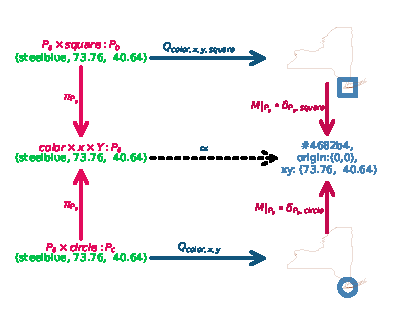
\includegraphics[width=\linewidth]{../paper/figures/compositor.pdf}
    \end{figure}
\end{frame}

\section{Implementation}
\begin{frame}<presentation:1|handout:1>{Implementation Choices: $\vartistc_{\dbasec} = \vartistc_{\gbasec}$}
    \begin{equation*}
        \begin{tikzcd}[ampersand replacement=\&, column sep=small]
            \cgamma{\opensetgc}{\vindexpullc\dtotalc\restriction_{\opensetgc}}
            \arrow[rr, "\vchannelc_{\gbasec}", color=artist]
            \arrow[rrrr, "\vartistc_{\gbasec}", bend left, color=artist]
            \&  \&
            \cgamma{\opensetgc}{\vindexpullc\vtotalc\restriction_{\opensetgc}}
            \arrow[rr, "\vmarkc_{\gbasec}", color=artist] \&  \&
            \imartist{\opensetgc}{\gtotalc\restriction_{\opensetgc}}
            \arrow[dd, "\vindexpushc", color=functor] \\
             \&  \&   \&  \& \\
            \cgamma{\openset}{\dtotalc\restriction_{\opensetc}}
            \arrow[rr, "\vchannelc_{\dbasec}", color=artist]
            \arrow[rrrr, "\vartistc_{\dbasec}", bend right, color=artist]
            \arrow[uu, "\vindexpullc", color=functor] \&  \&
            \cgamma{\openset}{\vtotalc\restriction_{\opensetc}}
            \arrow[rr, "\vmarkc_{\dbasec}", color=artist ]
            \arrow[uu, "\vindexpullc", , color=functor] \&  \&
            \imartist{\opensetc}{\vindexpushc\gtotalc\restriction_{\opensetc}}
            \end{tikzcd}
    \end{equation*}
\end{frame}

\begin{frame}[allowframebreaks]{References}
    \printbibliography
\end{frame}
\end{document}